\begin{figure}[H]
\centering
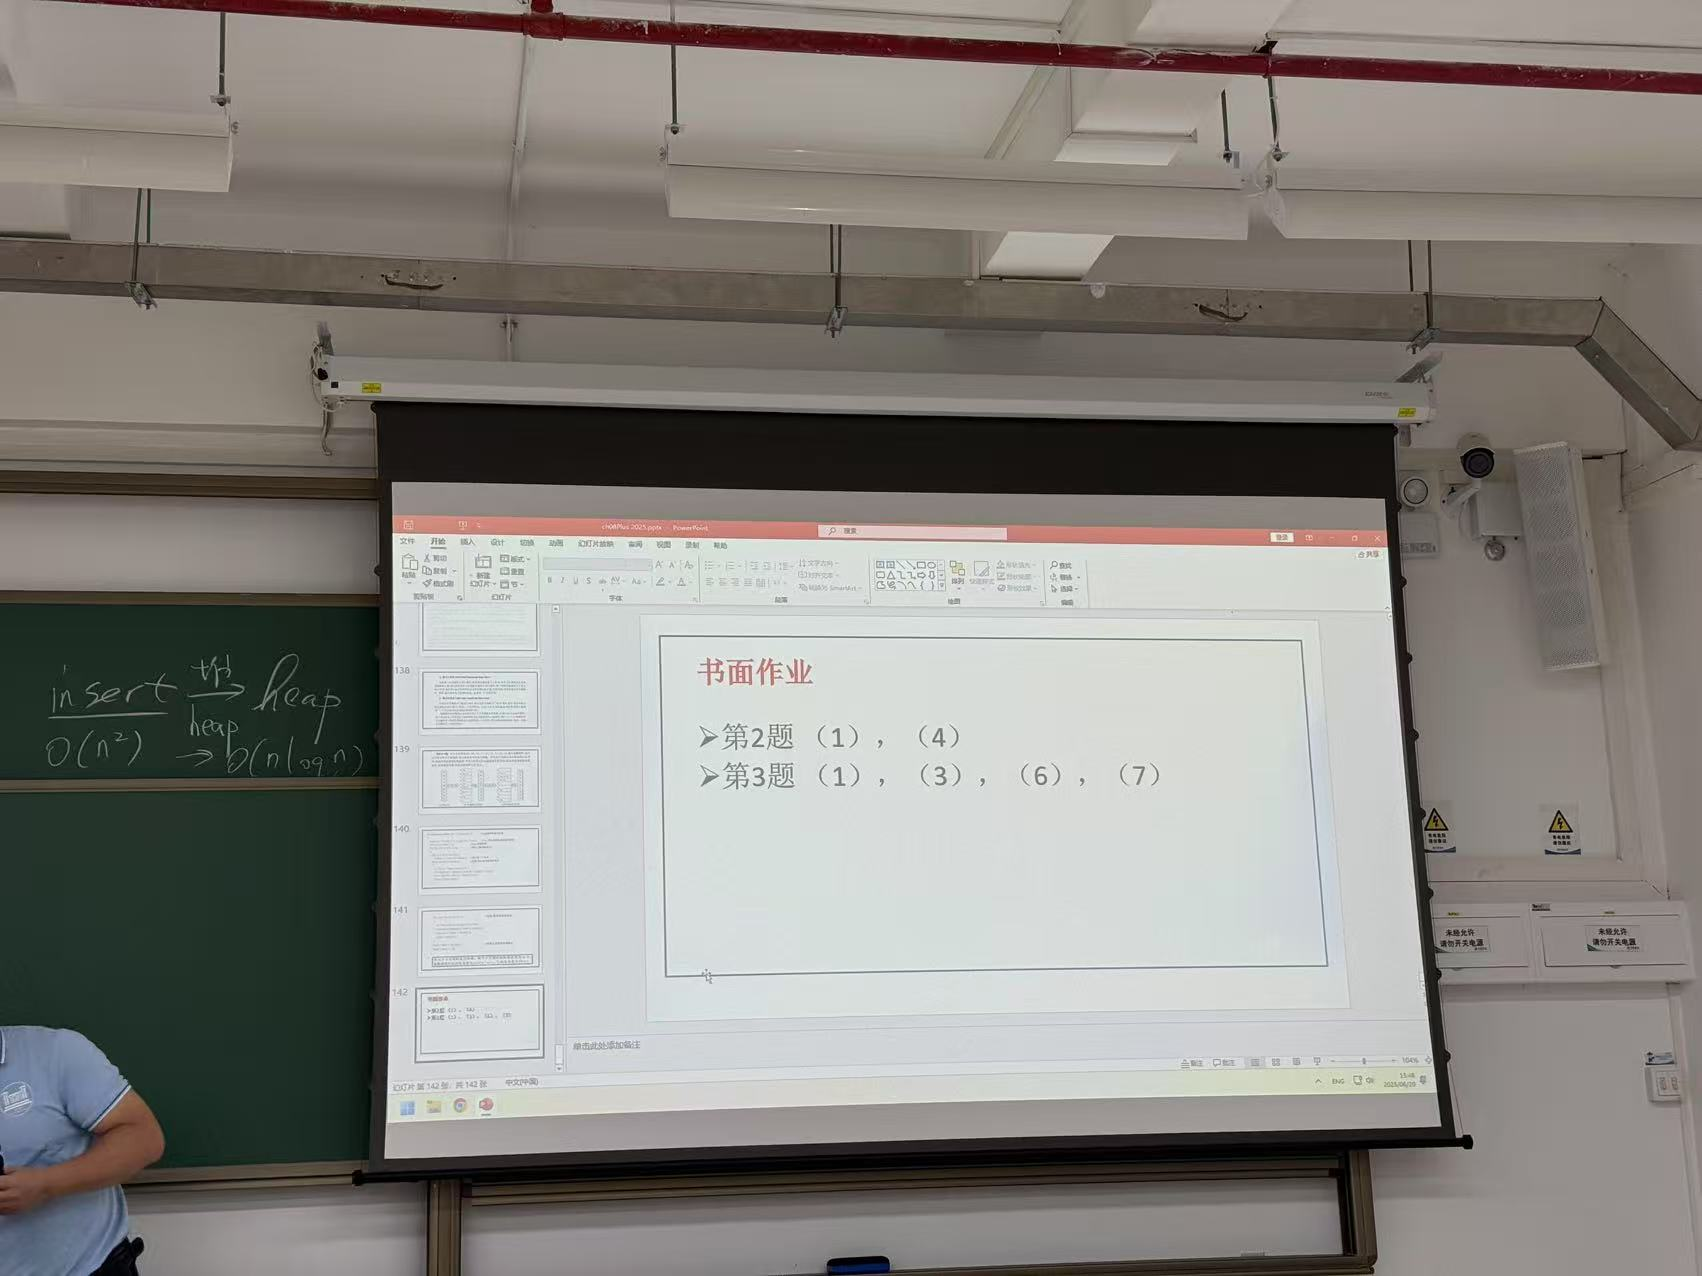
\includegraphics[width=\textwidth]{1983673f3597d785ee6edc6c81a330aa.jpg}
% \caption{}
\label{}
\end{figure}

\begin{exercise}
\begin{figure}[H]
\centering
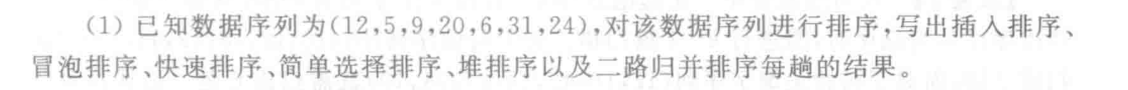
\includegraphics[width=\textwidth]{1-hw10-2025062308.png}
% \caption{}
\label{}
\end{figure}
\end{exercise}
\begin{figure}[H]
\centering
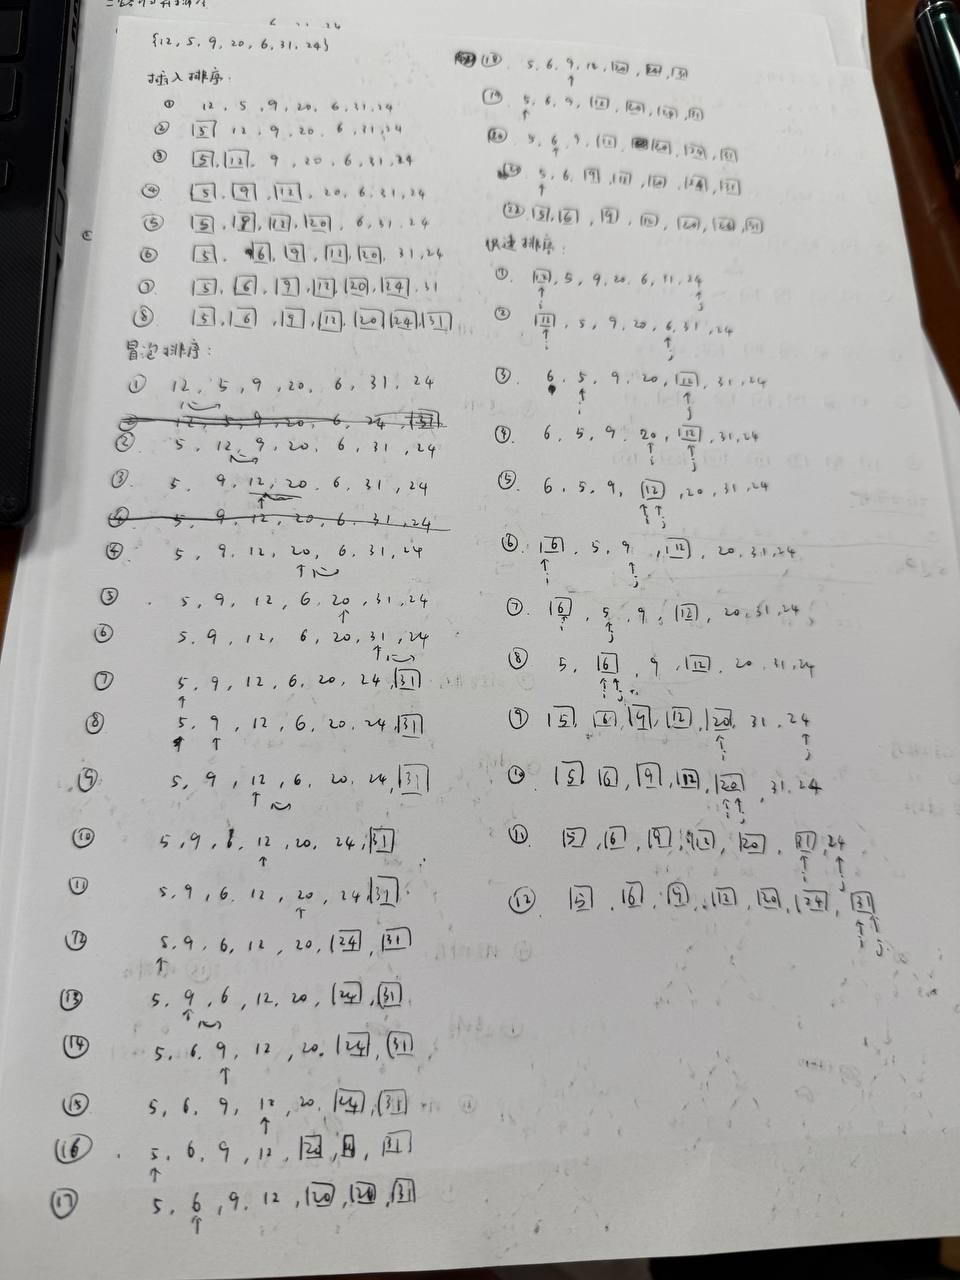
\includegraphics[width=\textwidth]{hw10-2025062312.png}
% \caption{}
\label{}
\end{figure}
\begin{figure}[H]
\centering
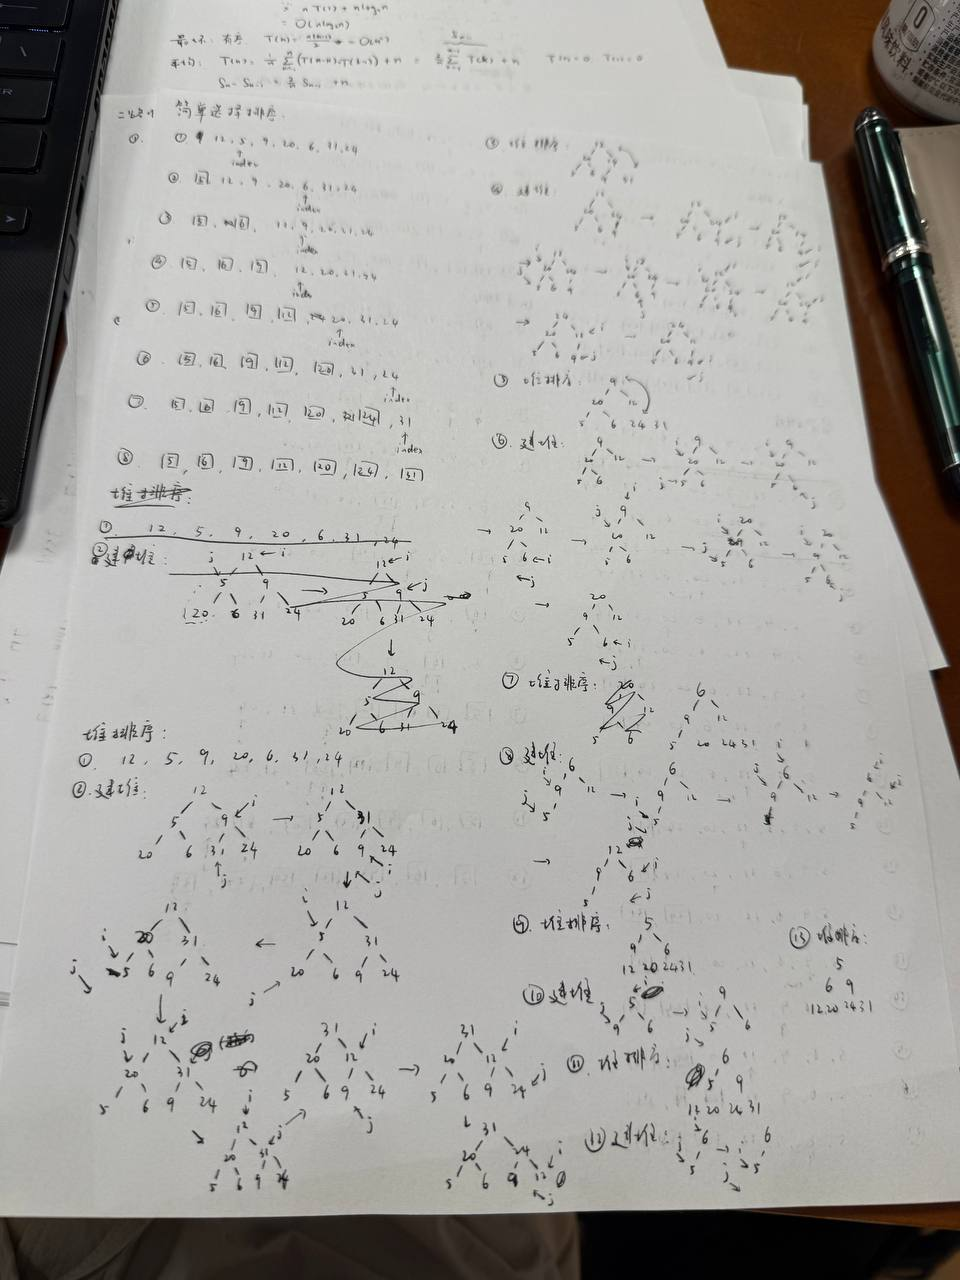
\includegraphics[width=\textwidth]{1-hw10-2025062312.png}
% \caption{}
\label{}
\end{figure}
\begin{figure}[H]
\centering
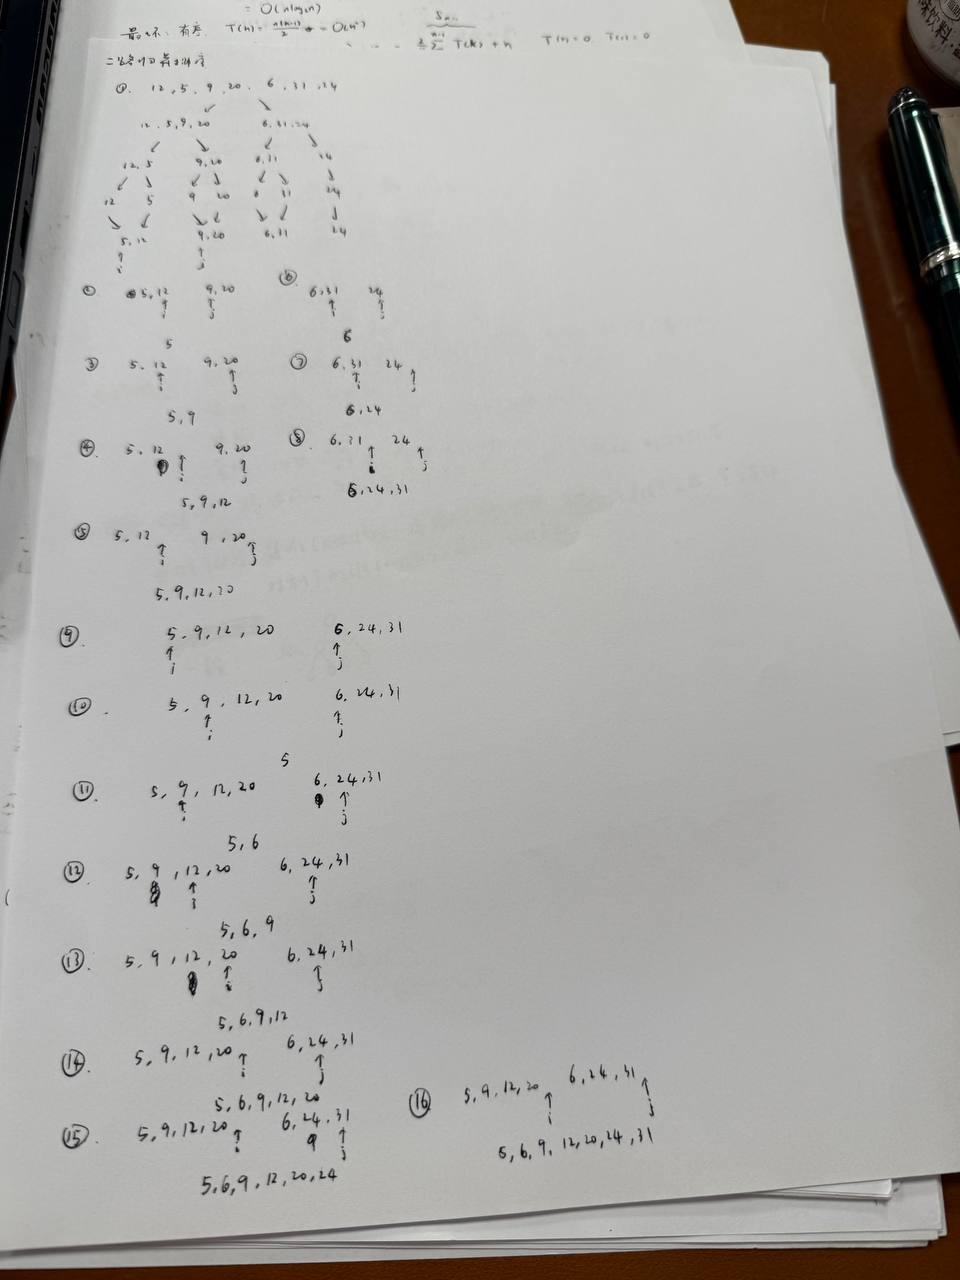
\includegraphics[width=\textwidth]{2-hw10-2025062312.png}
% \caption{}
\label{}
\end{figure}

\begin{exercise}
\begin{figure}[H]
\centering
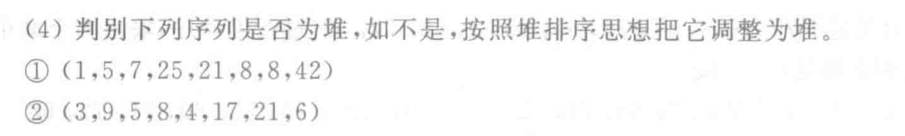
\includegraphics[width=\textwidth]{2-hw10-2025062308.png}
% \caption{}
\label{}
\end{figure}
\end{exercise}
\begin{figure}[H]
\centering
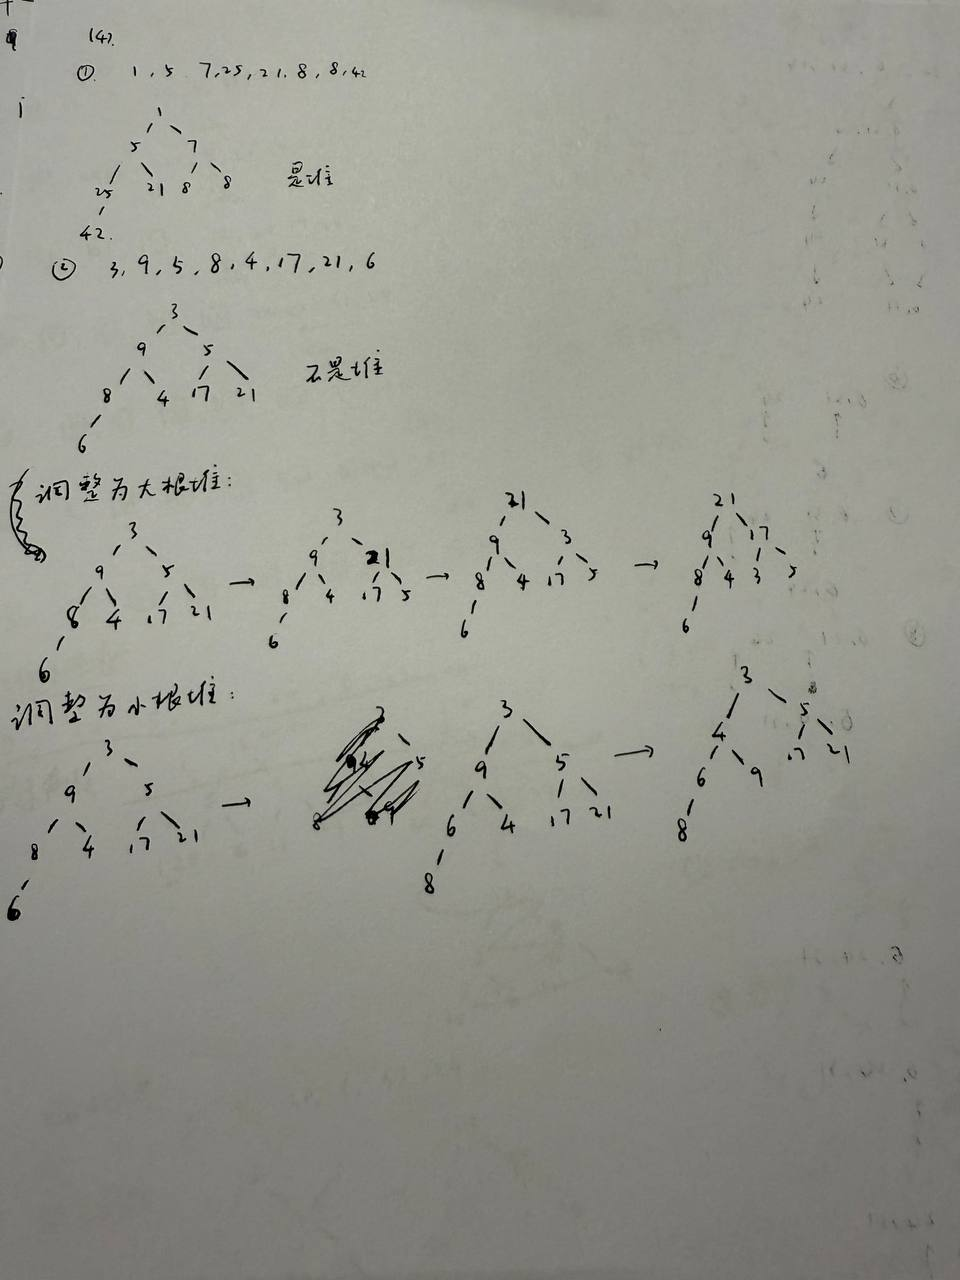
\includegraphics[width=\textwidth]{hw10-2025062314.png}
% \caption{}
\label{}
\end{figure}

\begin{exercise}
\begin{figure}[H]
\centering
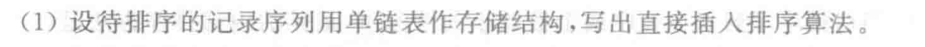
\includegraphics[width=\textwidth]{3-hw10-2025062308.png}
% \caption{}
\label{}
\end{figure}
\end{exercise}
\begin{lstlisting}
Input: 单链表头指针 head
Output: 指向已排序的单链表头指针 head

Algorithm:
1. 暂存 q = head,指向无序区的第一个结点
2. 将 q 存入有序区,q = q->next
3. 将 p 指向有序区的最后一个结点,即判定 p->next == q
4. 将 q->data 与 head 到 p 的每一个结点(有序区)的值相比较,插入到正确的位置.
5. 然后 p->next = p->next->next
6. 以此类推,直到 p->next == NULL
\end{lstlisting}
\begin{exercise}
\begin{figure}[H]
\centering
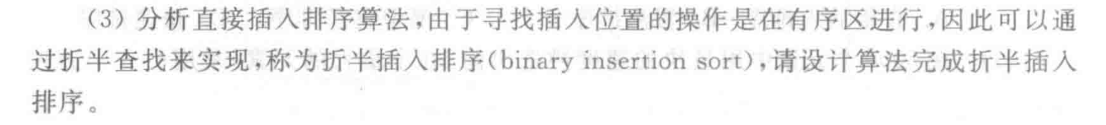
\includegraphics[width=\textwidth]{4-hw10-2025062308.png}
% \caption{}
\label{}
\end{figure}
\end{exercise}
\begin{lstlisting}
Input: 待排序的数组 a,长度 n
Output: 已排序的数组 a

Algorithm:
1. 当有序区长度为 k 时,考虑 a[k].
2. 先通过折半查找找到 a[k] 应该插入的位置. 令 i = 0, j = k-1, 若 a[(j+i)/2] <= a[k],则 i = (j+i)/2;否则 j = (j+i)/2,直到 i == j.
3. 然后 temp = a[k]; a[i+1] = a[i+2]; ... ; a[k-1] = a[k]; a[i] = temp; k++
4. 以此类推,直到 k == n

\end{lstlisting}
\begin{exercise}
\begin{figure}[H]
\centering
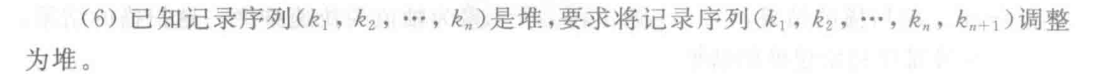
\includegraphics[width=\textwidth]{5-hw10-2025062308.png}
% \caption{}
\label{}
\end{figure}
\end{exercise}
\begin{lstlisting}

Algorithm HeapInsertAndSort(A, n, k_new)
    // Input: 
    //   A[0..n-1] - Initial max heap array of n elements
    //   n - Number of elements in the initial heap
    //   k_new - New element k_{n+1} to be inserted
    // Output: Sorted array A[0..n] in ascending order

    // Step 1: Insert k_new at the end and adjust to maintain max heap
    A[n] ← k_new              // Add new element at the end
    i ← n                     // Start from the last position
    while i > 0 do
        parent ← ⌊(i - 1) / 2⌋
        if A[i] > A[parent] then
            swap A[i] with A[parent]
            i ← parent
        else
            break
        end if
    end while

    // Step 2: Heap sort to get sorted sequence
    for i ← n downto 1 do
        swap A[0] with A[i]    // Move max element to the end
        heapSize ← i - 1       // Reduce heap size
        j ← 0                  // Start from root
        while true do
            left ← 2 * j + 1
            right ← 2 * j + 2
            smallest ← j
            if left < heapSize and A[left] < A[smallest] then
                smallest ← left
            end if
            if right < heapSize and A[right] < A[smallest] then
                smallest ← right
            end if
            if smallest = j then
                break
            end if
            swap A[j] with A[smallest]
            j ← smallest
        end while
    end for

    // Return the sorted array
    return A[0..n]
end Algorithm


\end{lstlisting}
\begin{exercise}
\begin{figure}[H]
\centering
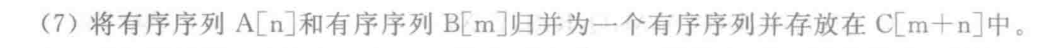
\includegraphics[width=\textwidth]{6-hw10-2025062308.png}
% \caption{}
\label{}
\end{figure}
\end{exercise}
\begin{lstlisting}
Input: A[n], B[m]
Output: C[m+n]

Algorithm:
i = 0; j = 0
while (i < n && j < m)
    if (a[i] >= b[j])
        c[i+j] = a[i]; i++
    else 
        c[i+j] = b[j]; j++
    end if
end while

while (i == n && j < m)
    c[i+j] = b[j]; j++
while (j == m && i < n)
    c[i+j] = a[i]; i++

\end{lstlisting}